
\pagestyle{plain} 	%numéro de page centré en pieds de page

\setcounter{tocdepth}{4}     % Dans la table des matieres


\section{Modelisation des Reseaux de Capteurs sans fil}

\subsection{Modele de base}

\begin{figure}[h]
\centering
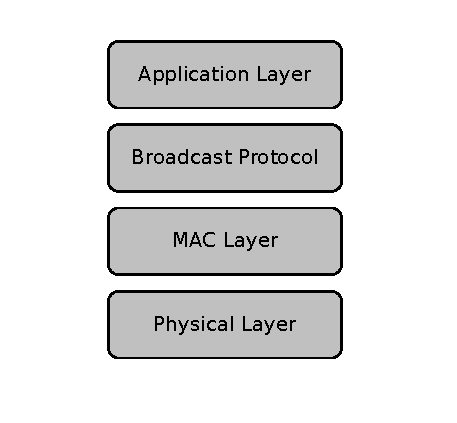
\includegraphics[scale=0.9]{source/layer.pdf}
\caption{\label{Layer} Les couches dans les WSNs}
\end{figure}

Pour l'étude et la conception d'algorithmes dans les reseaux de capteurs sans fil(WSN), il est indispensable de définir le probleme precis, d'établir un cadre rigoureux,formel et sans ambiguités. Au vue de la figure \ref{Layer}, notre étude se 
placera dans la couche 'Broadcast Protocols'. Nous ne développerons pas la couche MAC ni la couche applications\\

  La modélisation de base des réseaux de capteurs sans fil \textbf{$M_1$}:
\begin{itemize}
 \item Tout les capteurs sont identiques (batterie,portée, capacité de calcul..).
 \item le reseau est initialement connexe (chaque capteur est lié directement ou indirectement à tout les autres).
 \item Dans un plan euclidien à deux dimensions ( distance euclidienne)
 \item Sans mobilité des capteurs : nous supposerons que les capteurs sont fixes
 \item Sans ajout de capteurs: Le reseau comprends un nombre fixe de capteurs $n$. Aucun ajout de capteurs en court de fonctionnement n'est possible.
 \item Dans des conditions de transmition de message ideale: aucunes interferences entre les messages, pas de perturbations des ondes, systeme d'identifiants unique.
 \item Fiabilité des capteurs: aucune pannes possible, energie des capteurs infinie \\

\end{itemize}

  La modélisation \textbf{$M_2$} prendra de plus en compte :
\begin{itemize}
 \item Chaque capteur a une énergie initiale $E_i$ donnée. L'envoie de message consomme une quantité fonction du modèle énergétique choisie.Un capteur est eliminé lorsqu'il n'a plus d'énergie ou que son energie restante ne permet plus
aucun envoie de message. Les capteurs ne tombent pas en panne en raison d'autres facteurs.   
 \item L'ajout de capteurs: Le reseau comprends un nombre variable de capteurs $n$. Les ajouts de capteurs en court de fonctionnement sont possibles.\\
 
\end{itemize}

  La modélisation \textbf{$M_3$} prendra de plus en compte :
\begin{itemize}
 \item Les capteurs peuvent tomber en panne en raisons de divers facteurs. Une loi de probabilité modélise ce phénomene  .   
 \item La mobilité des capteurs.\\
 
\end{itemize}


  Un WSN peut etre représenté par un graphe $G= (V,E,\gamma)$ ou $V$ est un ensemble de noeuds(capteurs), $\gamma$ le rayon d'émission maximum et $E \subseteq V \textsuperscript{2}$ l'ensemble des arêtes représentants les communications
 possibles entre les capteurs: $(u,v)$ appartient à $E$ signifie que $u$ peut envoyer un  message à $v$. On note $ n=|V| $ la taille du WSN. En fait les éléments de E dépendent de la position des capteurs ainsi que de leur portée.Nous 
supposerons que tout les capteurs ont la même portée maximale notée $\gamma$. Nous noterons $d_e(u,v)$ la distance euclidienne dans $\mathbb{R} \textsuperscript{2}$ entre $u$ et $v$.
$$E = \{ (u,v) \in V ^{2} \mid d(u,v) \leq R \}$$

%%%%%%%%%%%%%%%%%%%%%%%%%%%%%%%%%%Graphe unité
\begin{mydef}
 On appelera $G= (V,E,\gamma)$ le \textit{graphe unité} du WSN et $\gamma$ son rayon de communication.
\end{mydef}

%%%%%%%%%%%%%%%%%%%%%%%%%%%%%%%%%%ùVoisinage
\begin{mydef}
On note le 1-voisinage de $u$ :$N_1(u) = \{ v \in V  \mid (u,v) \in E \}$ \\
On note le 2-voisinage de $u$ :$N_2(u) = \{ v \in V \mid  \exists w \in V :\{(u,w);(w,v)\} \in E ^2\}$ \\
On note le $k$-voisinage de $u$, $k \in \mathbb{N} : N_k(u) = \{ v \in V  \mid \exists $ un chemin $c (u,v): |c| \leq k\}$  On parlera de 1- 2- et k-voisins de $i$ pour désigner des noeud appartenant respectivement à $N_1(i),
N_2(i),N_k(i)$. \\
Soit $A \subseteq V$, on note $N(A) = \{ v \in V\textbackslash  A \mid \forall u\in A,(u,v) \in E \}$ \\
\end{mydef}

\begin{mydef}
 On appelera diametre de G $diametre_G=\max_{i,j\in \textlbrackdbl 1,n \textrbrackdbl,i<j}(d_G(i,j))$.
\end{mydef}
 
\begin{figure}[H]
\centering
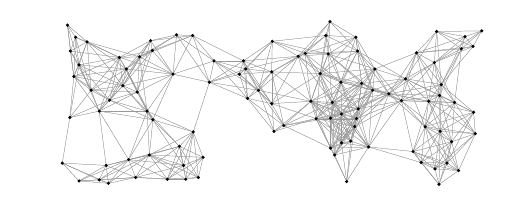
\includegraphics[scale=0.5]{source/graph1.png}
\caption{Graphe unité}
\end{figure} 


\begin{mydef}
 Le degré de $ u $ est le nombre  $N(u)=|N_1(u)|$.\\
 On note $d(u,v)$ la distance entre $ u $ et $ v $ : $d_G(u,v)= \min_{k \in \mathbb{N}}(k \mid v \in N_k(u))$
\end{mydef}

\begin{mydef}%%Densité, distance moyenne
 La densité de G est la moyenne des degrés:$$N_G=\sum_{i=1}^n{\frac1n N(i)}$$
 La distance de G est la moyenne des distances entre toutes paires de sommets:$$d_G=\sum_{i,j\in \textlbrackdbl 1,n \textrbrackdbl,i<j}{\frac1n d_G(i,j)}$$
 La distance euclidienne de G est la moyenne des distances euclidienne entre toutes paires de sommets:$$d_e(G)=\sum_{i,j\in \textlbrackdbl 1,n \textrbrackdbl,i<j}{\frac1n d_e1(i,j)}$$

\end{mydef}

\subsection{Modele energetique}
\subsubsection{Energie d'un capteur}
Tout les capteurs $i$ offrant les même caracteristiques, ils peuvent modifier leur rayon d'émission $r_i$ entre $r_i=0$ et $r_i=\gamma$.
Nous considererons que chaque capteur $i$ a une énergie initiale $E_{init}=\beta$.
Nous noterons $E_i$ l'energie restante de $i$.
L'envoie d'un message de $i$ avec un rayon $r$ coute $$E(r)=\begin{cases} r^\alpha + c & \text{si }i\neq j \\ 0 & \text{sinon}  \end{cases}$$
L'envoie d'un message de $i$ à $j$ ($d_e(i,j)\leq \gamma$) coute  $ E_{ij}=E(d_e(i,j))$.
L'energie consommée lors de la réception de message, du traitement et des calculs propres aux capteurs est négligée.


\subsubsection{Energie globale}
\begin{mydef}
 L'énergie potentielle de G est la somme des énergies des capteurs :$$E_G=\sum_{i=1}^n{E_i}$$
 La consomation de  G est :$$C_G=n\beta - E_G$$
 Le cout moyen de transmition de  G est :$$c_G=E(d_e(G))$$

\end{mydef}

\subsection{Initialisation et mise à jour d'un capteur}
Un capteur 'prend naissance', c'est à dire débute son activité dès qu'il est en place dans le réseaux et ce automatiquement. Deux choix sont possibles: soit le capteur est immédiatement opérationel soit il nécessite une phase 
d'initialisation. Il existe donc deux type d'algorithmes: sans balisage (beaconless) et avec balisage. Les algorithmes 'beaconless' ne nécessitent pas de phase d'initialisation ni de mise à jour. Les nouveaux capteurs sont immédiatement 
opérationels mais n'ont aucune connaissance de leur environnement et notement de leur voisinage dans G. Dans les algorithmes avec balisage, tout capteur, lorsqu'il 'prend naissance' commence par une procédure d'initialisation et stocke en 
mémoire un certain nombre d'informations(voisins,groupe,topologie locale...). Au cour de l'algorithme, chaque noeud met périodiquement à jour ces informations.

The broadcast schemes may require different neighborhood information, which is reflected in the contents of messages sent by nodes
 when they move, 
react to topological changes, change activity 
status, or simply send periodically update messages. Commonly seen `hello' message may contain, in addition to its own ID, its position, one bit for dominating set status (one bit saying to neighbors whether or not node 
considers itself to be in dominating set), list of l-hop neighbors, its degree (number of its neighbors). Other content is also possible, such as list ofl- hop neighbors with their positions, or list of 2-hop neighbors,
 or even global network information. Global Position System (GPS) provides geographic location information (if required) to hosts in a wireless network by communication with a satellite network. Alternatively, nodes may 
measure time delays or signal strengths of incoming messages and determine the relative location of its neighbors.

Quelle type d'informations est utilisée dans l'algorithme: informations globale du reseau ou informations locales? La distinction entre global est local n'est pas toujours évidente. Des algorithmes centralisés peuvent etre implémentés
 d'une maniere distribuée en décidant par exemple d'un noeud possedant la connaissance globale du réseau.Sinon, au travers d'un échange séquentiel d'informations tres locales (1 ou 2-voisinage par example), chaque noeud peut combiner sa 
connaissance avec celle de ses voisins et ainsi obtenir une vision globale du réseau. Cepandant, une telle phase de propagation coute tres cher en terme de nombre de messages échangés et de temps.
Si le reseau est dynamique (mobilité des capteurs), maintenir une connaissance locale du reseau devient plus complexe tandis que tenir a jour la topologie globale de celui-ci devient impossible par le moyen cité précedement.Ainsi, 
la quantité et la nature des informations nécessaire au déroulement de l'algorithme sont une bonne mesure de la capacité d'adaptation du protocol à un environement dynamique.   

\begin{enumerate}
 \item \textbf{Global}:         protocol de broadcast, centralisé ou distribué nécessitant une connaissance globale du reseau(ex: BIP).
 \item \textbf{Quasi-global}:   protocol distribué de broadcast nécessitant une connaissance quasi-globale du reseau.
 \item \textbf{Quasi-local}:    protocol distribué nécessitant une connaissance du réseau principalement locale et occasionellement globale.
(ex: Cluster networks: tandis que les groupes peuvent etres construits de maniere locale , des reactions en chaines peuvent arrivées).
 \item \textbf{Local}: 		protocol distribué nécessitant une connaissance tres locale du réseau.Tout les algorithmes de 1 ou 2-voisinage appartienent à cette catégorie.
\end{enumerate}


\subsection{Broadcast}

Dans un WSN $G(V,E,\gamma)$, deux capteurs peuvent communiquer directment uniquement si ils sont 1-voisins dans G.
A cause de la perte de propagation des messages, le rayon de transmition est relativement limité, c'est pourquoi les communications doivent se faire par multi-sauts, parfois meme si le destinataire est a distance 1 dans le graphe 
unité(pour des raison énergetiques). Pour établir une connection entre deux noeud non voisins, les messages doivent effectues des sauts via des noeuds intermediaires. Dans un large WSN, il est bien trop difficile pour un capteur voulant
transmettre un message à un autre de trouver une route, à cause de l'absence d'infrastructures. Pour ce faire, il lance une procedure de requette de route DSR (Dynamic Source Routing) via un broadcast.
La procédure de Broadcast est un mécanisme fondamentale pour la propagation des données ainsi que pour la decouverte de route. C'est pourquoi, concevoir des algorithmes efficaces et economes en énergie est un probleme primordial 
dans les WSN. 





{%
\newcommand{\mc}[3]{\multicolumn{#1}{#2}{#3}}
\begin{center}
\begin{tabular}{|c|l}\cline{1-1}
\mc{2}{c}{\textbf{Notations}}\\\hline
$G(V,E,\gamma)$ & \mc{1}{c|}{Graphe unité}\\\hline
$n$ & \mc{1}{c|}{Nombre de capteur}\\\hline
$\gamma$ & \mc{1}{c|}{Rayon d'émission maximum}\\\hline
$\alpha$ & \mc{1}{c|}{constante de consommation énergetique}\\\hline
$c$ & \mc{1}{c|}{constante de consommation énergetique}\\\hline
$\beta$ & \mc{1}{c|}{Energie initiale des capteur}\\\hline
$E_i$ & \mc{1}{c|}{Energie restante de $i$}\\\hline
$E_{ij}$ & \mc{1}{c|}{Cout d'envoie d'un message de $i$ à $j$}\\\hline
$N(u) $& \mc{1}{c|}{Degre de u}\\\hline
$d_G(i,j)$ & \mc{1}{c|}{distance dans G entre $i$ et $j$}\\\hline
$d_e(i,j)$ & \mc{1}{c|}{distance euclidienne entre $i$ et $j$}\\\hline
$N_k(u)$ & \mc{1}{c|}{nombre de k-voisins de u }\\\hline
$N_G$ & \mc{1}{c|}{densité de G}\\\hline
$d_G$ & \mc{1}{c|}{distance de G}\\\hline
$d_e(G)$ & \mc{1}{c|}{distance euclidienne de G}\\\hline
$diametre_G$ & \mc{1}{c|}{diametre de G}\\\hline
\end{tabular}
\end{center}
}%


\section{Classification}\label{class}


\subsection{Elements de classification}

\begin{enumerate}
 \item  rayon de transmission fixe ou variable
 \item  probabiliste ou deterministe
 \item  basé sur les clusters
 \item  Grid Partitioning-Based Backbone
 \item  Clustering-Based Backbone
 \item  Connected Dominating Set (CDS)-Based Backbone
 \item  Activity scheduling and power-aware broadcasting
 \item  Broadcasting with directional antennas
 \item  Flooding scheme 
 \item  Probabilistic flooding
 \item  1-Hop Neighbor Knowledge Methods
 \item  Flooding with Self Pruning (FSP)
 \item  2-Hop or More Neighbor Knowledge Methods
 \item  Multipoint Relaying (MPRs)
 \item  Using Connected Dominating Set (CDS)
 \item  Area Based Methods.....................
 
\end{enumerate}

power saving, power control for TR, Blackbone,1,2,k-hop neighborhood, initialisation(beaconless), flooding, gossiping, clustering, coverage, probabilistic based, area based,selecting forwarding, nes, election, time out, optimal range,\\


Les éléments de classification cités ci dessous sont inspirés des articles \cite{stojmenovic2004},\cite{ingelrest2005},\cite{wu2003}


\subsubsection{Extensibilité}
Il est facile d'admettre que l'extensibilité d'un WSN est inversement proportionelle à la localité du protocol. Pour qu'un protocol soit extensible, il doit etre avant tout distribué et local: le comportement de chaque noeud bien qu'il
nécessite qu'une connaissance locale du reseau, permet d'atteindre l'objectif global. 

Intelligent and scalable broadcasting and activity scheduling solutions are based on the concept of dominating sets. Clusterheads and gateway nodes in a cluster structure define such a set, and were
 first `Intelligent' 
flooding solution proposed in literature. However, the node mobility either worsens the quality of the structure dramatically, or otherwise causes chain reaction (local changes in the structure could trigger global updates). 
Localized connected dominating set concepts, proposed recently, avoid such chain reaction, and have similar or better rebroadcast savings. Their maintenance does not require any communication overhead in addition to 
maintaining positions of neighboring nodes, or information about 2-hop neighbors. One such concept is based on covering of all 2-hop neighbors by a minimal set of l-hop neighbors. The other is based on creating a fixed 
dominating set, where nodes that do not have two unconnected neighbors, and nodes that are `covered' by one or two neighbors (each neighbor of a covered node is neighbor of one of nodes that cover it) are eliminated.
 Neighbor elimination was also applied (solely or in conjunction with other concepts), where nodes give up retransmitting if they are not aware of any neighbor that did not already receive the same message. This chapter
 will survey known techniques based on dominating sets, and will discuss their advantages and drawbacks.

\subsubsection{Connectivité}. Reliability is the ability of a broadcast protocol to reach all the nodes in the network. It can be considered at the network or at the medium access layer. We will classify protocols according to 
their network 
layer performance. That is, assuming that MAC layer is ideal (every message sent by a node reaches all its neighbors), location update protocol provides accurate desired information to all nodes about their neighborhood, and
 the network is connected, broadcast protocols can be reliable or unreliable. In a {\it reliable} protocol, every node in the network is reached. The set of nodes that rebroadcast message in a reliable broadcasting scheme 
define a connected dominating set. A dominating set $D(S)$ of a set $S$ is a set ofnodes such that each node fiom $S$ either belongs to $D(S)$ or has a neighboring node that belongs to $D(S)$. It is easy to observe that all
 nodes will receive the message if it is retransmitted only by nodes that belong to a connected dominating set. Connectivity provides propagation through the whole network, while domination assures reachability by all nodes.
 Broadcasting task can therefore be solved optimally by finding a connected dominating set of minimal size. Optimality here is measured by percentage of saved retransmissions in a reliable broadcasting scheme. Unfortunately,
 the problem of finding connected dominating set of minimal size is NP-complete, even if a node has global knowledge about the network [HH, LK, QVL]. Therefore one needs to apply heuristics to flood intelligently. Note also
 that a protocol that is reliable on the network layer may be very unreliable at the MAC layer, such as blind flooding. Excess messages in any protocol affect node's power and bandwidth available, thus the main goal is to
 describe a reliable broadcast protocol with minimal number of retransmissions, that is, to construct connected dominating set of minimal size. Note also that MAC layer cannot guarantee 100\% reliability, due to the hidden
 terminal problem (a node simultaneously receiving messages fiom two other nodes that are not aware of each other transmission) and the probabilistic nature of protocols used.

\subsubsection{Deterministe vs probabilistique}. A broadcast scheme may use probabilistic or deterministic protocol, based on whether or not a random number selection was used to make decisions. The random number usage here is
 limited to the network
 layer decision; the underlying medium access control (MAC) protocol may still use random back-off counters, for example, in a network layer deterministic scheme.



\subsubsection{Métriques}.The performance of broadcast protocols can be measured by variety of metrics. A commonly used metric is the number of message retransmissions (or the total power used in case of broadcasting with adjusted 
transmission
 radii) with respect to the number of nodes (alternatively, {\it rebroadcast savings}, a complementary measure, can be used). The next important metric is {\it reachability}, or the ratio of nodes connected to the source
 that received the broadcast message. Time delay or latency is sometimes used, which is the time needed for the last node to receive broadcast message initiated at the source. Note that retransmissions at MAC layer are 
normally deferred, to avoid message collisions. Some authors consider alternative more restricted indicator, whether or not the path fiom source to any node is always following a shortest path. This measure may be important
 ifused as part of routing scheme, since route paths are created during the broadcast process.



\subsection{Algorithmes sans balisage}
\subsubsection{Bling Flooding}
Le blind flooding ou broadcast aveugle est un algortihme glouton de broadcast. Lors de la reception d'un message par un noeud, si c'est la premiere fois qu'il le recoit, il le broadcast à ses voivins(avec le rayon maximum), sinon il
 ne fait rien.
\subsubsection{Algorithme ABBA}
'Area-based beaconless reliable broadcasting in
sensor networks'\cite{ABBA06}.

L'idée maitresse de ABBA est assez simple. Nous supposons que les noeuds n'ont aucunes connaissance de leur voisinage. Cepandant ceux ci connaissent leurs position géographique (GPS par exemple).
A la premiere réception d'un message broadcasté, le noeud initialise un timer. Avant expiration du timer, le noeud peut recoivoir d'autre copie du meme message. Chaque capteur a un rayon d'emission fixe $R$
et couvre une zone circulaire. Si un noeud $u$ recoit le meme message de differente source et que ces sources couvrent sa zone, alors $u$ ne retransmet pas le message.
Cela signifie que chaqun de ses voisins potentiel a déjà reçu le message. Si un noeud est couvert avant que son timer n'expire, il ne fait rien. Sinon il retransmet.
Comme chaque couverture est un cercle de rayon $R$, le critere de couverture peut etre simplifié: au lieu de s'interesser au disque entier, un noeud verifie uniquement si le perimetre de sa zone est couvert par 
ses voisins lui ayant envoyé le message. 



\begin{algorithm}[h]
\caption{ABBA}
\label{ABBA}
\begin{algorithmic}
\REQUIRE:
A source node $s$ broadcasts a message $M$
\STATE Reception  par  $u$ du message $M$ broadcasté par $s$
\STATE Set perimeter covered by the transmission of M;
\STATE Set timeout;
\REPEAT
    \STATE Wait until another copy of M is received or timeout expires;
    \IF {another copy is received}
	\STATE Update perimeter covered;
	\STATE update timeout;
    \ENDIF
\UNTIL{timeout expires;}
\IF {still uncovered}
    \STATE Retransmit;
\ENDIF
     \STATE Ignore further copies of M;

\end{algorithmic}
\end{algorithm}




\subsection{Algorthimes globaux}
\subsubsection{Algorithme BIP}
Article \cite{Wieselthier00}
\begin{itemize}
 \item Pas de mobilité.
 \item Conditions de transmition des messages ideale(aucunes interferences,identifiants donnés ...)  et fixe
 \item Desavantage des transmition longue portée: interférence, cout energetique ( rappelons que le modele de consommation energetique des noeuds est non linéaire par rapport au rayon à cause de l'attenuation du signal radio)
 \item Trouver le bon compromis entre le rayon de transmition et le nombre de messages circulant: un large rayon de transmittion coute cher mais ateind beaucoup de neouds; un court rayon cout tres peu cher mais 
augmente le nombre de messages. Facteurs de choix: topologie du reseau,



\end{itemize}

  L'algorithme de Prim est un algorithme permettant de construire un arbre
  couvrant minimal d'un graphe. 

  Le principe de l'algorithme de Prim est de construire l'arbre couvrant
  minimal arête par arête: pour ajouter une arête à un arbre partiellement
  construit, il considère l'ensemble des arêtes dont une extrémité est
  connectée à l'arbre déjà construit, et l'autre extrémité ne l'est pas, et
  il choisit dans cet ensemble une arête de poids minimal qu'il ajoute à
  l'arbre. L'algorithme commence avec un arbre couvrant contenant un n\oe
  ud et zéro arêtes, et ajoute successivement $n-1$ arêtes.

La formation d'un arbre couvrant de poids minimun dans BIP suit le meme principe dans le sens ou les noeuds sont un par un ajouté à l'arbre.
En fait, Bip utilise l'algorithme de Prim avec une difference fondamentale: au lieu d'utiliser les couts fixes $P_{ij}$ sur les aretes (demeurant inchangés au court de la procedure),
Bip actualise dynamiquement ces couts à chaques étapes($i.e$ à chaque ajout d'un noeud), ce qui traduit le fait que le cout d'ajout d'un neoud depends de ceux qui sont déja dans l'abre.
Par exemple,supposons que chaque noueds $i$ appartient a l'abre et un noeuds $j$ pas encore dans celui ci.Pour chaque noeuds $i$, et chaque noeuds $j$:
$$P_{ij'}=P_{ij}-P(i)$$
ou $P_{ij}$ est le cout reel de transmition et $P(i)$ le cout de broadcast de $i$ dans l'arbre ( $P(i)=0$ si $i$ est une feuille). $P_{ij'}$ represente donc le cout d'ajout de $j$ par un noeud appartenant au sous ensemble des feuilles
 directes de $i$(ou $i$ lui meme si c'est une feuille).La paire $\{i,j\}$ minimisant $P_{ij'}$ est selectionnée et $i$ transmet à $j$. Ainsi, un nouveau noeud est ajouté a chaque etape de l'algo.\\

.........................Algo a voir...........

\begin{algorithm}[h]
\caption{Procédure Construction BIP-Tree}
\label{algo_LBIP_sp}
\begin{algorithmic}
\REQUIRE:
\begin{itemize}
 \item Paramètres locaux : source du broadcast s, graphe G, Bip-tree B
 \item  Variables : \\
  -entier i, m, y\\
  -réel : v\\
  -ensemble : M\\
  -branche : pp\\
  -poids : d \\
\end{itemize}


\STATE  $B \leftarrow graphe_{vide}$
\STATE  $M \leftarrow Ensemble_{vide}$
  \FOR{ $i=0 \to  N$} 
    \STATE $d[i] \leftarrow P_si$
    \STATE $pp[i] \leftarrow s$ 
    \STATE $M \leftarrow Ajouter (i,M)$
  \ENDFOR
  \STATE $M \leftarrow Supprimer (s,M)$
  \WHILE {$M \neq Ensemble_{vide}$}
   \STATE $m \leftarrow Choisir (M,d)$
   \STATE $M \leftarrow Supprimer (m,M)$
   \STATE $z \leftarrow pp[m]$
   \STATE $v \leftarrow coût (m,z,G)$
   \STATE $T \leftarrow Ajout arête <m,z> de coût v à T$
   \FOR{ $i = 1 \to d° m \in G$} 
     \STATE $y \leftarrow← i ième_succ_de m dans G$
     \IF{ $y  M et (cout(m,y,G) < d[y]$)}
       \STATE $d[y] \leftarrow coût(m,y,G)$
       \STATE $pp[y] \leftarrow m$
     \ENDIF
    \ENDFOR
\ENDWHILE


\end{algorithmic}
\end{algorithm}

Contairement a Prim qui garantie l'optimalité de l'abre couvrant en termes de cout total,
Bip de construit pas forcement un arbre de poids minimum.


\subsection{Algorithmes de 2-voisinages}
\subsubsection{Algorithme LBIP}
`Localized Broadcast Incremental Power Protocol for Wireless Ad Hoc Networks' :\cite{Ingelrest04}

\begin{algorithm}[h]
\caption{LBIP setup phase}
\label{algo_LBIP_sp}
\begin{algorithmic}

\FOR{each node $N_i$}
	\STATE Broadcast a HELLO message
\ENDFOR

\STATE On receiving a message, put the sender in the 1-hop neighborhood

\FOR{each node $N_i$}
	\STATE Broadcast a HELLO message which contains the $N_i$ 1-hop neighborhood to compute the $N_i$ 2-hops neighborhood
\ENDFOR

\COMMENT{each node has a BIP tree of its 2-hops neighborhood}

\end{algorithmic}
\end{algorithm}



\begin{algorithm}[h]
\caption{LBIP}
\label{algo_LBIP}
\begin{algorithmic}

\STATE The source node $s$ sends a packet which contains instructions for relayer nodes
\IF{A node $u$ receives a packet from a node $v$ for the first time :}
	\IF{The packet contains some instructions for u}
		\STATE $u$ starts constructing a BIP tree within its own 2-hop neighborhood with ranges previously computed
	\ENDIF
\ENDIF

\end{algorithmic}
\end{algorithm}

\subsubsection{Algorithme RRS}
\cite{RNG03}
\subsubsection{Algorithme DLBIP}
\cite{Baert07}
\subsubsection{Algorithme RBOP}
\cite{cartigny2005}
\subsubsection{Algorithme LBOP}
\cite{cartigny2005}
\subsubsection{Algorithme DLBOP}
\cite{DLBOP04}
\subsubsection{Algorithme TR-LBOP}
\cite{TRLBOP}
\subsubsection{Algorithme FONIA}




\subsection{Probalistics}


\subsubsection{Algorithme BWGOSSIP}
\cite{lutzeler2011}
\subsubsection{Algorithme Duty-Cycle-Aware Broadcast in WSN }
\cite{Wang09},\cite{Wang10}
\subsubsection{Algorithme HEED}
\cite{Younis04}
\subsubsection{Algorithme WMH}
\cite{WMH05}
\subsubsection{Algorithme IRRIGATOR  Firework}
\cite{orecchia2004}
\subsubsection{Algorithme ML2B}
\cite{zhaobroadcast}
\subsubsection{Algorithme MLE}
\cite{Cheng06}
\subsubsection{Algorithme MPR}

\subsubsection{Algorithme Power Adaptive Broadcasting with Local Information}
\cite{chen2003}



\subsection{Protocoles}
\subsubsection{NES}

\newpage
\subsection{Synthèse}



\newpage

\begin{figure}[H]
\centering
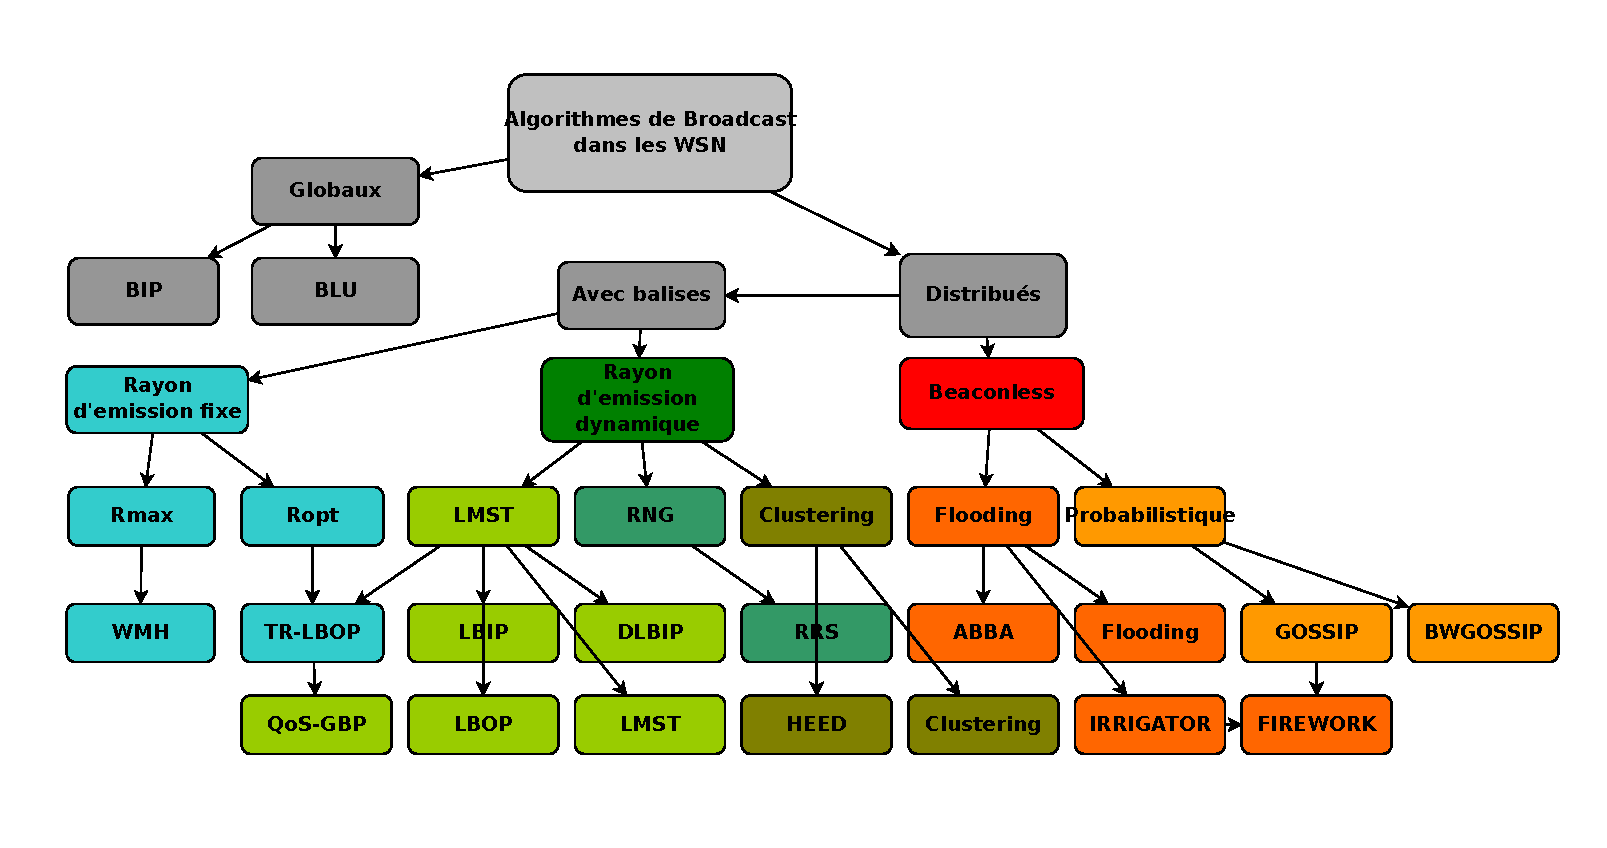
\includegraphics[scale=1,angle=90]{source/classification}
\caption{Description, Figure 1 : Graphe de synthèse}
\end{figure} 

\subsection{Lifetime}
Les definitions et critères de durée de vie d'un WSN sont tirés des articles \cite{Dietrich09},\cite{Baert06},\cite{Elleithy11}.


\subsubsection{Durée de vie du reseau, problématique}
\subsubsection{Energy-Efficiency (EE)}
\subsubsection{Time To First Fail (TTFF)}
\subsubsection{Operative Nodes Percentage (ONP)}
\subsubsection{Monitored Interest Points Percentage (MIPP)}
\subsubsection{The time there is at least a certain fraction $\beta$ of surviving nodes in the network }
\subsubsection{The time until all nodes have been drained of their energy }
\subsubsection{K-coverage: the time the area of interest is covered by at least k nodes }
\subsubsection{100 $\textperthousand$}
a. The time each target is covered by at least one node  ;
b. The time the whole area is covered by at least one node  ;

\subsubsection{$\alpha$-coverage}
a. The accumulated time during which at least $\alpha$ portion of the region is covered by
at least one node ;
b. The time until the coverage drops below a predefined threshold $\alpha$ (until last drop
below threshold)  ;
c. The continuous operational time of the system before either the coverage or
delivery ratio first drops below a predefined threshold ;

\subsubsection{The number of successful data-gathering trips}
\subsubsection{The number of total transmitted messages }
\subsubsection{The percentage of nodes that have a path to the base station}
\subsubsection{Expectation of the entire interval during which the probability of guaranteeing connectivity and k-coverage simultaneously is at least $\alpha$}
\subsubsection{The time until connectivity or coverage are lost}
\subsubsection{The time until the network no longer provides an acceptable event detection ratio}
\subsubsection{The time period during which the network continuously satisfies the application requirement}
\subsubsection{min(t1, t2, t3)}
with t1: time for cardinality of largest connected component of
communication graph to drop below c1 $\times$ n(t), t2: time for n(t) to drop below c2 $\times$ n, t3:
time for the covered volume to drop below c3 $\times$ l d .
